\label{motivation}
As described in \autoref{intro:clustering} the process of FAK clustering and its effect upon activation, especially on an atomistic scale, are still not understood and part of current research. In this thesis the results of MD simulations with the Martini force field (see \autoref{subsub:coarsegraining}) are presented, which address the clustering process of FAK molecules. In this context Martini is a necessary simplification due to the large number of particles in systems containing sever FAK molecules.\\
\\
However previous work in the group \autocite{sara} obtained difficulties in the use of Martini for simulations of FAK on a \pip{} containing membrane. In some simulations equivalent to setup 3 (see \autoref{setup:setup3}) except for an external force the protein rapidly changed its inclination to the membrane. In the following part this shall be characterised by the angle $\beta$ between the z-axis and the vector connecting F1 and F2, $\vec{d}_F$.
\begin{equation}
\cos\left(\beta\right) = \frac{\vec{d}_{F, z}}{d_F},\quad d_F = \left|\vec{d}_F\right|
\end{equation}
\textcite{sara} simulated five different copies for $10\,\si{\micro\second}$ each. The resulting distributions of the angle can be seen in \autoref{motiv:sarascurves}. Exemplary the red line shows a mean value of $90\,\si{\deg}$, which is what meant with a falling of FAK in the following part. The angle changed in less than $50\,\si{\nano\second}$ and stayed constant for the remaining simulation time.\\
There are several reasons why this is rather an artefact of the Martini force field than a possible binding pose of FAK to the membrane as suggested by \textcite{pap002}. The first one is, that FAK falls to both extensive sites, which means that the key residues for an interaction of the extensive site of the kinase with the membrane proposed by \textcite{pap002} are located on top of the FAK and not on the side of the membrane. Indeed contact analysis showed, that virtually all residues on the surface (in both, FERM domain and kinase) were interacting with the membrane. Another one is, that this behaviour was not observed in equivalent all atom simulations in C36 ($1.5\,\si{\micro\second}$ in total). Here only two maxima were observed around $8\,\si{\deg}$ and around $20\,\si{\deg}$, the largest observed angle was $40\,\si{\deg}$.\\
\\
In the course of this project several experiments were made to understand the cause of this falling, e. g. to review the binding of the basic patch in Martini, which is presented in \autoref{results:umbrella}. However the reason could not have proven beyond doubt. In order to still perform reasonable simulations of multiple FAK an external force was applied to each FAK molecule. This is called stabilizing force in the following parts.\\
The force is acting onto F1 and F2 parallel to the z-axis and is proportional to the deviation of their z-distance $\Delta z$ from a reference distance $z_0$. An illustration of the force can be found in \autoref{motiv:forceillustr}. For the determination of $z_0$ only the green and the blue distribution from \autoref{motiv:sarascurves} were considered, because the large angles observed in the other distributions have not been observed in C36 simulations. The mean value of $\vec{d}_{F, z}$ for these two distributions is $2.228\,\si{\nano\metre}$, which was therefore set as $z_0$. %TODO: get force constant out of distribution
\textit{@Csaba: sorry, but how did we get this force constant of 1000 out of the distributions?}\\
\\
%
%
%
\begin{figure}
	\subcaptionbox{\label{motiv:sarascurves}}[0.49\textwidth]{
		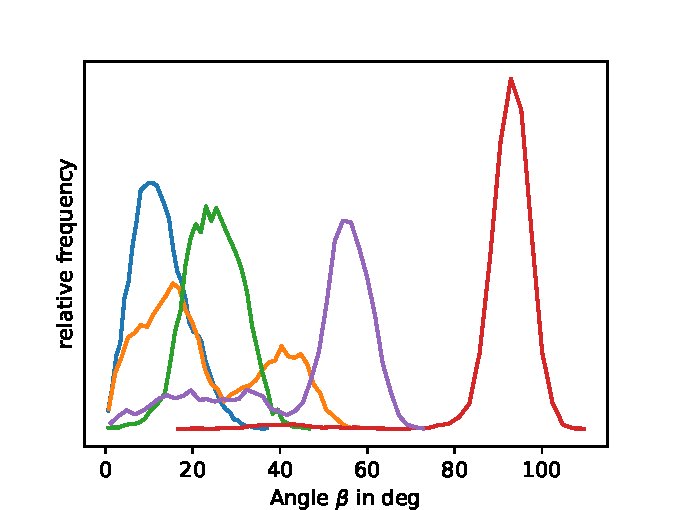
\includegraphics[height=5cm]{figures/introduction/sara_angles}
	}\hfill%
	\subcaptionbox{\label{motiv:forceillustr}}[0.49\textwidth]{
		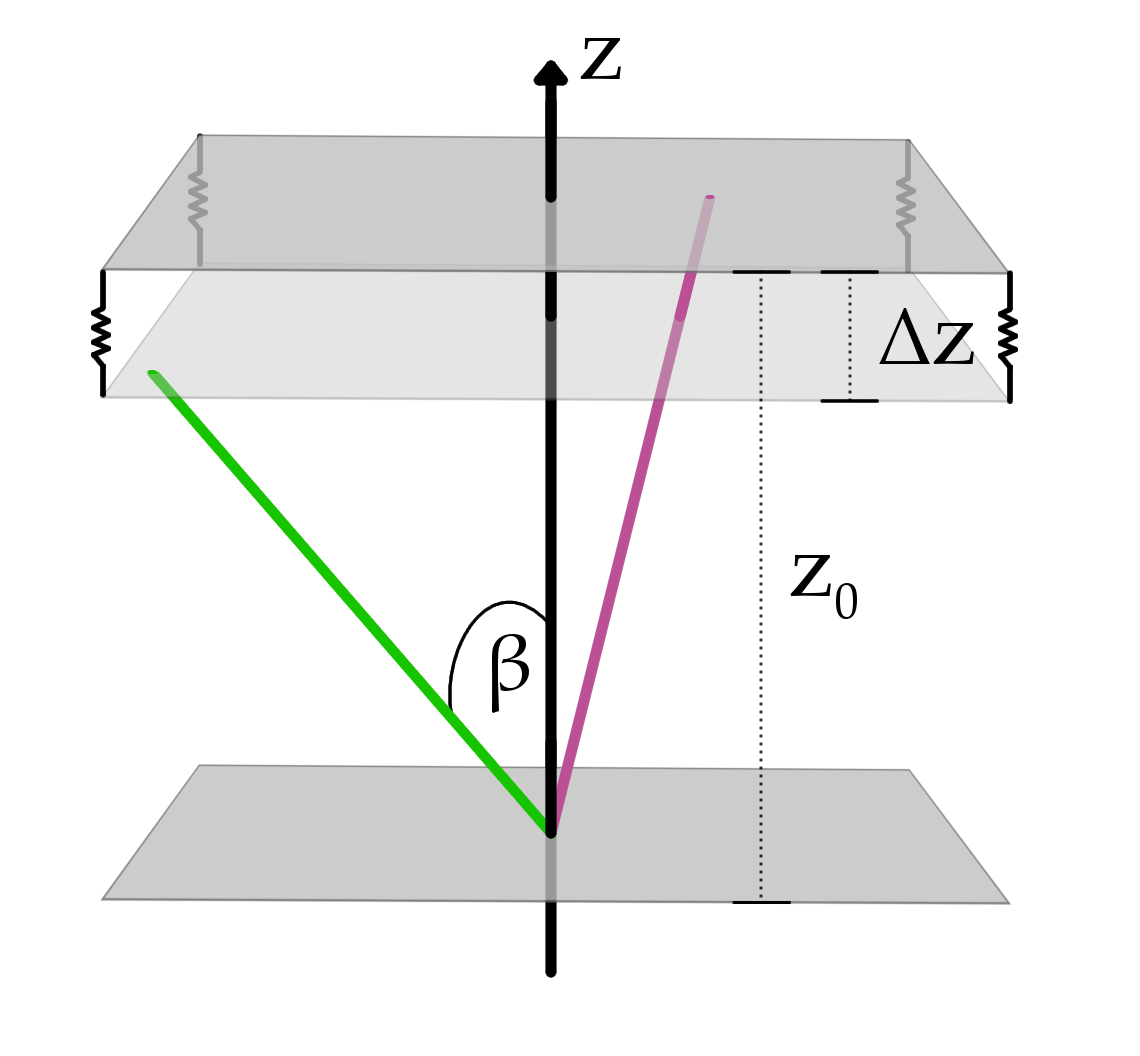
\includegraphics[height=5cm]{figures/introduction/forceapproach}
	}%
	\nicecaption{Inclination angle of FAK}{(\subref{motiv:sarascurves}): Distributions of $\beta$ obtained by \textcite{sara}. The red curve shows the distribution for a fallen FAK. (\subref{motiv:forceillustr}): Illustration of the applied force. Pink and green line represents possible orientations of $\vec{d}_{F, z}$. The force is proportional to $\Delta z$.}
\end{figure}
%
%
%
In the following two chapters the used methods, i.e. MD simulation, are explained and the used setups introduced. Afterwards the obtained results are presented. For this purpose FAK in solution and FAK bound to \pip{} are analysed and compared to known information from experiments or other simulations. Also the impacts of the stabilizing force onto the simulations are commented. At last the focus is set on interactions between multiple FAK molecules.

